\documentclass{standalone}
\usepackage{tikz}
\usetikzlibrary{patterns, positioning}

\begin{document}
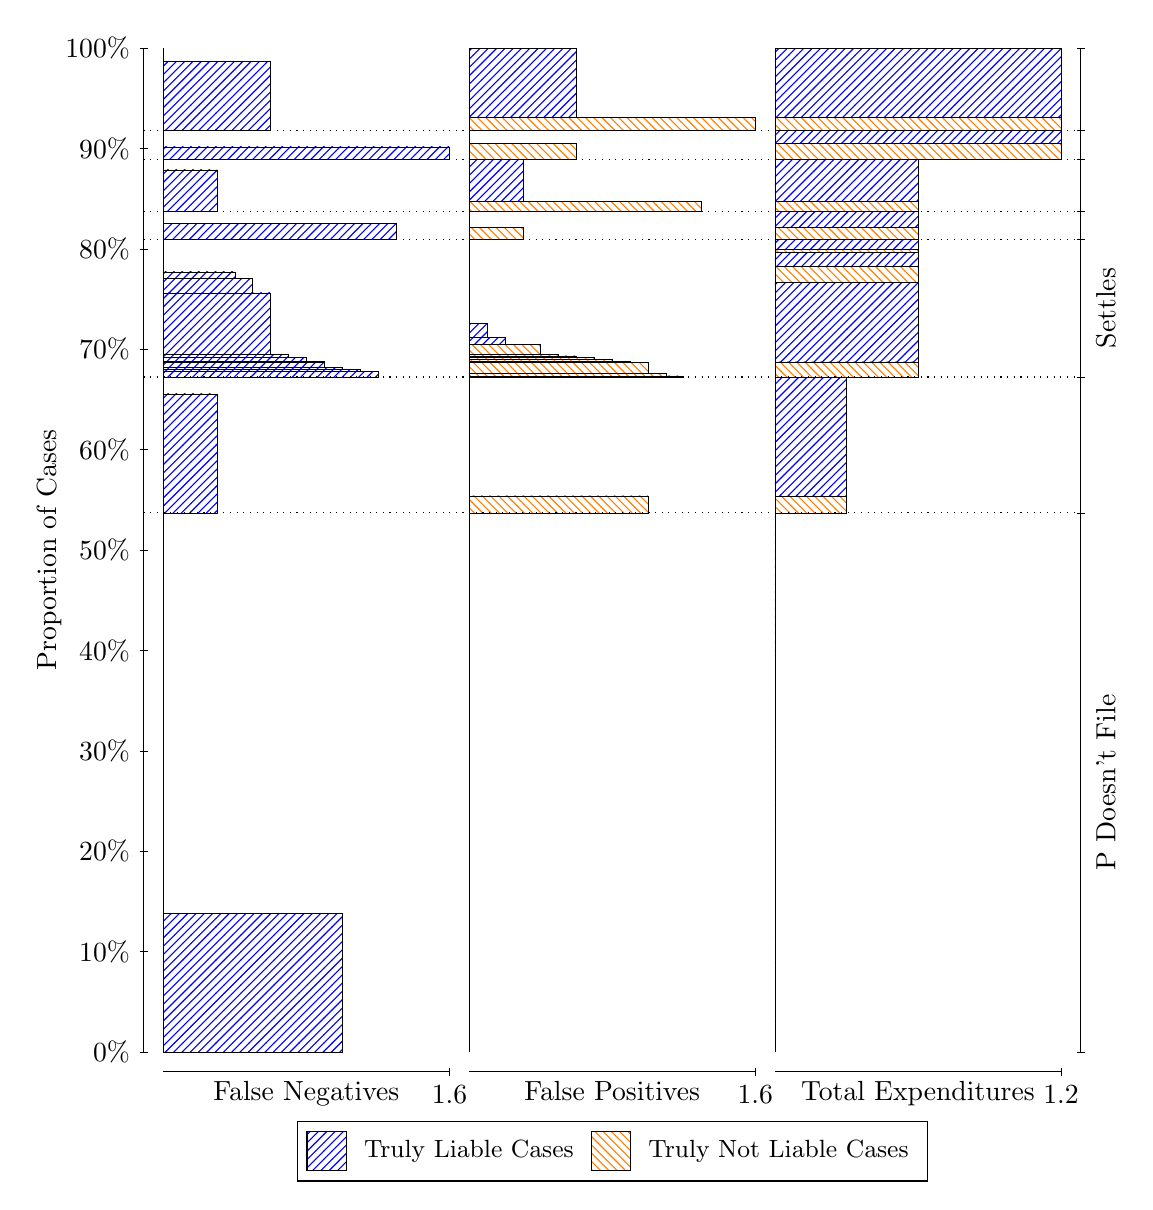
\begin{tikzpicture}
\draw[black, very thin] (1.5,1.75) -- (1.5,14.5);
\node[rotate=90, anchor=center] at (0.3, 8.125) {Proportion of Cases};
\draw[black, very thin] (1.45,1.75) -- (1.55,1.75);
\node[anchor=east] at (1.45, 1.75) {0\%};
\draw[black, very thin] (1.45,3.025) -- (1.55,3.025);
\node[anchor=east] at (1.45, 3.025) {10\%};
\draw[black, very thin] (1.45,4.3) -- (1.55,4.3);
\node[anchor=east] at (1.45, 4.3) {20\%};
\draw[black, very thin] (1.45,5.575) -- (1.55,5.575);
\node[anchor=east] at (1.45, 5.575) {30\%};
\draw[black, very thin] (1.45,6.85) -- (1.55,6.85);
\node[anchor=east] at (1.45, 6.85) {40\%};
\draw[black, very thin] (1.45,8.125) -- (1.55,8.125);
\node[anchor=east] at (1.45, 8.125) {50\%};
\draw[black, very thin] (1.45,9.4) -- (1.55,9.4);
\node[anchor=east] at (1.45, 9.4) {60\%};
\draw[black, very thin] (1.45,10.675) -- (1.55,10.675);
\node[anchor=east] at (1.45, 10.675) {70\%};
\draw[black, very thin] (1.45,11.95) -- (1.55,11.95);
\node[anchor=east] at (1.45, 11.95) {80\%};
\draw[black, very thin] (1.45,13.225) -- (1.55,13.225);
\node[anchor=east] at (1.45, 13.225) {90\%};
\draw[black, very thin] (1.45,14.5) -- (1.55,14.5);
\node[anchor=east] at (1.45, 14.5) {100\%};

\draw[black, very thin] (13.4,1.75) -- (13.4,14.5);
\draw[black, very thin] (13.35,1.75) -- (13.45,1.75);
\node[anchor=west] at (13.35, 1.75) {};
\draw[black, very thin] (13.35,8.5975) -- (13.45,8.5975);
\node[anchor=west] at (13.35, 8.5975) {};
\draw[black, very thin] (13.35,10.322) -- (13.45,10.322);
\node[anchor=west] at (13.35, 10.322) {};
\draw[black, very thin] (13.35,12.074) -- (13.45,12.074);
\node[anchor=west] at (13.35, 12.074) {};
\draw[black, very thin] (13.35,12.421) -- (13.45,12.421);
\node[anchor=west] at (13.35, 12.421) {};
\draw[black, very thin] (13.35,13.081) -- (13.45,13.081);
\node[anchor=west] at (13.35, 13.081) {};
\draw[black, very thin] (13.35,13.455) -- (13.45,13.455);
\node[anchor=west] at (13.35, 13.455) {};
\draw[black, very thin] (13.35,14.5) -- (13.45,14.5);
\node[anchor=west] at (13.35, 14.5) {};

\draw[black, very thin, pattern color=blue, pattern=north east lines] (1.75,1.75) rectangle (4.0208,3.508);
\draw[black, very thin, pattern color=orange, pattern=north west lines] (1.75,3.508) rectangle (1.75,8.5975);
\draw[black, very thin, pattern color=blue, pattern=north east lines] (1.75,8.5975) rectangle (2.4312,10.108);
\draw[black, very thin, pattern color=orange, pattern=north west lines] (1.75,10.108) rectangle (1.75,10.322);
\draw[black, very thin, pattern color=blue, pattern=north east lines] (1.75,10.322) rectangle (4.475,10.394);
\draw[black, very thin, pattern color=blue, pattern=north east lines] (1.75,10.394) rectangle (4.2479,10.418);
\draw[black, very thin, pattern color=blue, pattern=north east lines] (1.75,10.418) rectangle (4.0208,10.446);
\draw[black, very thin, pattern color=blue, pattern=north east lines] (1.75,10.446) rectangle (3.7937,10.509);
\draw[black, very thin, pattern color=blue, pattern=north east lines] (1.75,10.509) rectangle (3.7937,10.518);
\draw[black, very thin, pattern color=blue, pattern=north east lines] (1.75,10.518) rectangle (3.5667,10.572);
\draw[black, very thin, pattern color=blue, pattern=north east lines] (1.75,10.572) rectangle (3.3396,10.611);
\draw[black, very thin, pattern color=blue, pattern=north east lines] (1.75,10.611) rectangle (3.1125,11.39);
\draw[black, very thin, pattern color=blue, pattern=north east lines] (1.75,11.39) rectangle (2.8854,11.571);
\draw[black, very thin, pattern color=blue, pattern=north east lines] (1.75,11.571) rectangle (2.6583,11.657);
\draw[black, very thin, pattern color=orange, pattern=north west lines] (1.75,11.657) rectangle (1.75,12.074);
\draw[black, very thin, pattern color=blue, pattern=north east lines] (1.75,12.074) rectangle (4.7021,12.274);
\draw[black, very thin, pattern color=orange, pattern=north west lines] (1.75,12.274) rectangle (1.75,12.421);
\draw[black, very thin, pattern color=blue, pattern=north east lines] (1.75,12.421) rectangle (2.4312,12.951);
\draw[black, very thin, pattern color=orange, pattern=north west lines] (1.75,12.951) rectangle (1.75,13.081);
\draw[black, very thin, pattern color=blue, pattern=north east lines] (1.75,13.081) rectangle (5.3833,13.244);
\draw[black, very thin, pattern color=orange, pattern=north west lines] (1.75,13.244) rectangle (1.75,13.455);
\draw[black, very thin, pattern color=blue, pattern=north east lines] (1.75,13.455) rectangle (3.1125,14.333);
\draw[black, very thin, pattern color=orange, pattern=north west lines] (1.75,14.333) rectangle (1.75,14.5);
\draw[black, very thin, pattern color=orange, pattern=north west lines] (5.6333,1.75) rectangle (5.6333,6.8395);
\draw[black, very thin, pattern color=blue, pattern=north east lines] (5.6333,6.8395) rectangle (5.6333,8.5975);
\draw[black, very thin, pattern color=orange, pattern=north west lines] (5.6333,8.5975) rectangle (7.9042,8.8124);
\draw[black, very thin, pattern color=blue, pattern=north east lines] (5.6333,8.8124) rectangle (5.6333,10.322);
\draw[black, very thin, pattern color=orange, pattern=north west lines] (5.6333,10.322) rectangle (8.3583,10.337);
\draw[black, very thin, pattern color=orange, pattern=north west lines] (5.6333,10.337) rectangle (8.1313,10.37);
\draw[black, very thin, pattern color=orange, pattern=north west lines] (5.6333,10.37) rectangle (7.9042,10.505);
\draw[black, very thin, pattern color=orange, pattern=north west lines] (5.6333,10.505) rectangle (7.6771,10.519);
\draw[black, very thin, pattern color=orange, pattern=north west lines] (5.6333,10.519) rectangle (7.45,10.542);
\draw[black, very thin, pattern color=orange, pattern=north west lines] (5.6333,10.542) rectangle (7.2229,10.575);
\draw[black, very thin, pattern color=orange, pattern=north west lines] (5.6333,10.575) rectangle (6.9958,10.59);
\draw[black, very thin, pattern color=orange, pattern=north west lines] (5.6333,10.59) rectangle (6.7687,10.608);
\draw[black, very thin, pattern color=orange, pattern=north west lines] (5.6333,10.608) rectangle (6.5417,10.739);
\draw[black, very thin, pattern color=blue, pattern=north east lines] (5.6333,10.739) rectangle (6.0875,10.825);
\draw[black, very thin, pattern color=blue, pattern=north east lines] (5.6333,10.825) rectangle (5.8604,11.006);
\draw[black, very thin, pattern color=blue, pattern=north east lines] (5.6333,11.006) rectangle (5.6333,12.074);
\draw[black, very thin, pattern color=orange, pattern=north west lines] (5.6333,12.074) rectangle (6.3146,12.221);
\draw[black, very thin, pattern color=blue, pattern=north east lines] (5.6333,12.221) rectangle (5.6333,12.421);
\draw[black, very thin, pattern color=orange, pattern=north west lines] (5.6333,12.421) rectangle (8.5854,12.551);
\draw[black, very thin, pattern color=blue, pattern=north east lines] (5.6333,12.551) rectangle (6.3146,13.081);
\draw[black, very thin, pattern color=orange, pattern=north west lines] (5.6333,13.081) rectangle (6.9958,13.291);
\draw[black, very thin, pattern color=blue, pattern=north east lines] (5.6333,13.291) rectangle (5.6333,13.455);
\draw[black, very thin, pattern color=orange, pattern=north west lines] (5.6333,13.455) rectangle (9.2667,13.622);
\draw[black, very thin, pattern color=blue, pattern=north east lines] (5.6333,13.622) rectangle (6.9958,14.5);
\draw[black, very thin, pattern color=orange, pattern=north west lines] (9.5167,1.75) rectangle (9.5167,6.8395);
\draw[black, very thin, pattern color=blue, pattern=north east lines] (9.5167,6.8395) rectangle (9.5167,8.5975);
\draw[black, very thin, pattern color=orange, pattern=north west lines] (9.5167,8.5975) rectangle (10.425,8.8124);
\draw[black, very thin, pattern color=blue, pattern=north east lines] (9.5167,8.8124) rectangle (10.425,10.322);
\draw[black, very thin, pattern color=orange, pattern=north west lines] (9.5167,10.322) rectangle (11.333,10.513);
\draw[black, very thin, pattern color=blue, pattern=north east lines] (9.5167,10.513) rectangle (11.333,11.528);
\draw[black, very thin, pattern color=orange, pattern=north west lines] (9.5167,11.528) rectangle (11.333,11.722);
\draw[black, very thin, pattern color=blue, pattern=north east lines] (9.5167,11.722) rectangle (11.333,11.909);
\draw[black, very thin, pattern color=orange, pattern=north west lines] (9.5167,11.909) rectangle (11.333,11.94);
\draw[black, very thin, pattern color=blue, pattern=north east lines] (9.5167,11.94) rectangle (11.333,12.074);
\draw[black, very thin, pattern color=orange, pattern=north west lines] (9.5167,12.074) rectangle (11.333,12.221);
\draw[black, very thin, pattern color=blue, pattern=north east lines] (9.5167,12.221) rectangle (11.333,12.421);
\draw[black, very thin, pattern color=orange, pattern=north west lines] (9.5167,12.421) rectangle (11.333,12.551);
\draw[black, very thin, pattern color=blue, pattern=north east lines] (9.5167,12.551) rectangle (11.333,13.081);
\draw[black, very thin, pattern color=orange, pattern=north west lines] (9.5167,13.081) rectangle (13.15,13.291);
\draw[black, very thin, pattern color=blue, pattern=north east lines] (9.5167,13.291) rectangle (13.15,13.455);
\draw[black, very thin, pattern color=orange, pattern=north west lines] (9.5167,13.455) rectangle (13.15,13.622);
\draw[black, very thin, pattern color=blue, pattern=north east lines] (9.5167,13.622) rectangle (13.15,14.5);
\draw[black, dotted] (1.5,8.5975) -- (13.4,8.5975);
\draw[black, dotted] (1.5,10.322) -- (13.4,10.322);
\draw[black, dotted] (1.5,12.074) -- (13.4,12.074);
\draw[black, dotted] (1.5,12.421) -- (13.4,12.421);
\draw[black, dotted] (1.5,13.081) -- (13.4,13.081);
\draw[black, dotted] (1.5,13.455) -- (13.4,13.455);
\draw[black, very thin] (1.75,1.5) -- (5.3833,1.5);
\node[anchor=north] at (3.5667, 1.5) {False Negatives};
\draw[black, very thin] (5.3833,1.45) -- (5.3833,1.55);
\node[anchor=north] at (5.3833, 1.45) {1.6};

\draw[black, very thin] (5.6333,1.5) -- (9.2667,1.5);
\node[anchor=north] at (7.45, 1.5) {False Positives};
\draw[black, very thin] (9.2667,1.45) -- (9.2667,1.55);
\node[anchor=north] at (9.2667, 1.45) {1.6};

\draw[black, very thin] (9.5167,1.5) -- (13.15,1.5);
\node[anchor=north] at (11.333, 1.5) {Total Expenditures};
\draw[black, very thin] (13.15,1.45) -- (13.15,1.55);
\node[anchor=north] at (13.15, 1.45) {1.2};

\node[black, centered, rotate=90] at (13.72, 5.1737) {P Doesn't File};

\node[black, centered, rotate=90] at (13.72, 11.198) {Settles};





\draw (7.449999999999999,1.5) node[draw=none] (baseCoordinate) {};
\begin{scope}[align=center]
        \matrix[scale=0.5, draw=black, below=0.5cm of baseCoordinate, nodes={draw}, column sep=0.1cm]{
            \node[rectangle, draw, minimum width=0.5cm, minimum height=0.5cm, pattern=north east lines, pattern color=blue] {}; &
            \node[draw=none, font=\small] (B) {Truly Liable Cases}; &
            \node[rectangle, draw, minimum width=0.5cm, minimum height=0.5cm, pattern=north west lines, pattern color=orange] {}; &
            \node[draw=none, font=\small] (B) {Truly Not Liable Cases}; \\
            };
\end{scope}

\end{tikzpicture}
\end{document}